\documentclass[12pt]{book}
\usepackage{palatino}
\usepackage{epsfig}

\setlength{\topmargin}{0in}
\setlength{\oddsidemargin}{0.2in}
\setlength{\evensidemargin}{0.2in}
\setlength{\textwidth}{6.4in}
\setlength{\textheight}{10.5in}
\setlength{\parindent}{0in}
\setlength{\parskip}{0in}
\pagestyle{empty}

\begin{document}
  
  \begin{center}
    {\LARGE \bf DUMNEZEIASCA LITURGHIE\\
      \vspace{0.1in}
      \^{I}n Duminici \c{s}i S\u{a}rb\u{a}tori}
  \end{center}

  \vspace{0.3in}

  {\bf Preotul:} Binecuv\^{a}ntat\u{a} este \^{i}mp\u{a}r\u{a}\c{t}ia
  Tat\u{a}lui \c{s}i a Fiului \c{s}i a Sf\^{a}ntului Duh, acum \c{s}i
  pururea \c{s}i \^{i}n vecii vecilor.

  {\bf Cantorul:}
  \begin{figure}[h]
    \begin{center}
      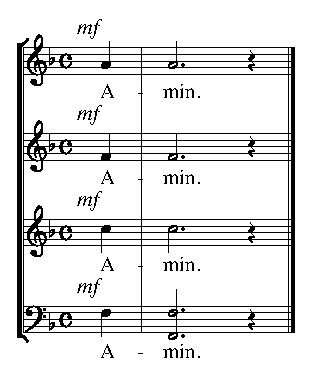
\epsfig{file=amin_1.eps}
    \end{center}
  \end{figure}

  \begin{center}
    {\large \bf ECTENIA MARE\\
      Glas 8}
  \end{center}

  {\bf Preotul:} Cu pace, Domnului s\u{a} ne rug\u{a}m.

  {\bf Cantorul:}
  \begin{figure}[h]
    \begin{center}
      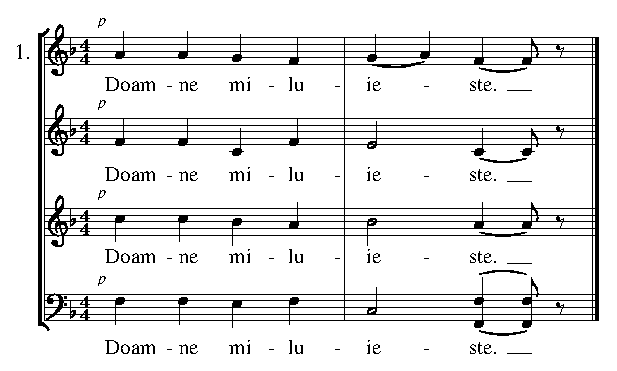
\epsfig{file=dm_1.eps}
    \end{center}
  \end{figure}

  \pagebreak
  \pagestyle{myheadings} \markright{\hfill \small } \setcounter{page}{2}

  {\bf Preotul:} Pentru pacea de sus \c{s}i pentru m\^{a}ntuirea
  sufletelor noastre, Domnului s\u{a} ne rug\u{a}m.

  {\bf Cantorul:}
  \begin{figure}[h]
    \begin{center}
      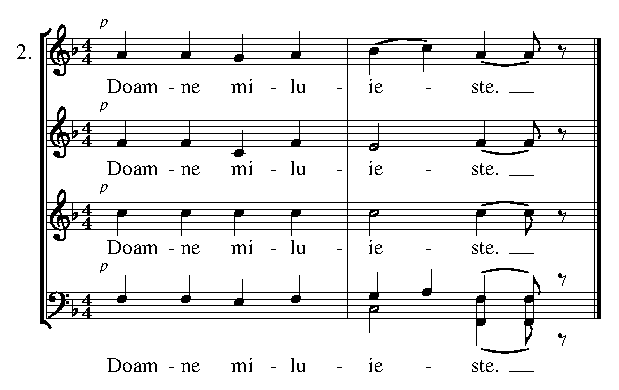
\epsfig{file=dm_2.eps}
    \end{center}
  \end{figure}

  {\bf Preotul:} Pentru pacea a toat\u{a} lumea, pentru bun\u{a}starea
  sfintelor lui Dumnezeu biserici \c{s}i pentru unirea tuturor,
  Domnului s\u{a} ne rug\u{a}m.

  {\bf Cantorul:}
  \begin{figure}[h]
    \begin{center}
      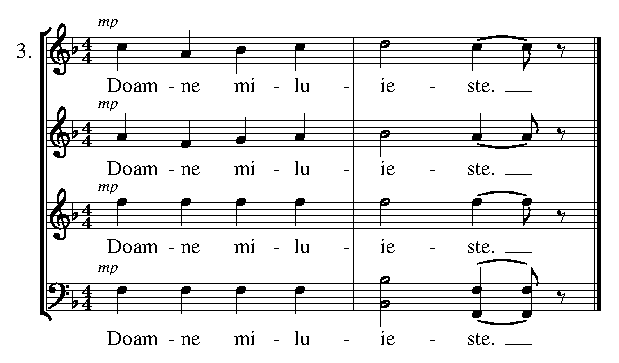
\epsfig{file=dm_3.eps}
    \end{center}
  \end{figure}

  \pagebreak

  {\bf Preotul:} Pentru sf\^{a}nt\u{a} biserica aceasta \c{s}i pentru
  cei ce cu credin\c{t}\u{a}, cu evlavie \c{s}i cu fric\u{a} de
  Dumnezeu intr\u{a} \c{s}i se roag\u{a} \^{i}ntr-\^{a}nsa, Domnului
  s\u{a} ne rug\u{a}m.

  {\bf Cantorul:}
  \begin{figure}[h]
    \begin{center}
      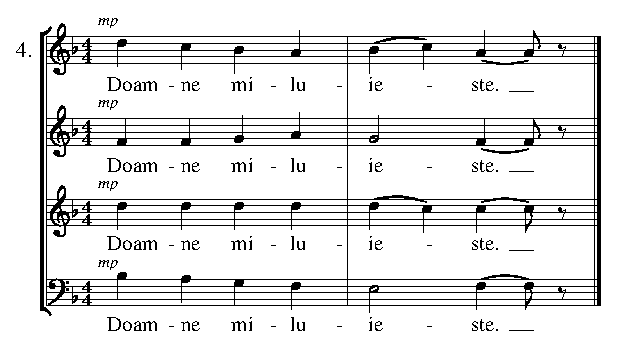
\epsfig{file=dm_4.eps}
    \end{center}
  \end{figure}

  {\bf Preotul:} Pentru Prea Sfin\c{t}itul Episcopul nostru {\em
  (nume)} (Arhiepiscop, Mitropolit, Patriarh), pentru cinsita
  preo\c{t}ime \c{s}i \^{i}ntru Hristos diaconime, pentru tot clerul
  \c{s}i poporul, Domnului s\u{a} ne rug\u{a}m.

  {\bf Cantorul:}
  \begin{figure}[h]
    \begin{center}
      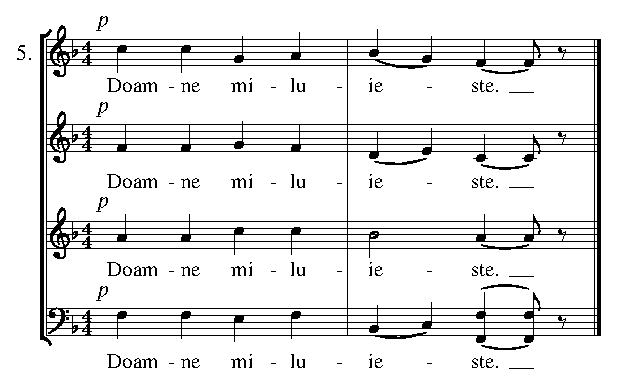
\epsfig{file=dm_5.eps}
    \end{center}
  \end{figure}

  \pagebreak

  {\bf Preotul:} Pentru Pre\c{s}edintele \c{t}\u{a}rii nostre {\em
  (nume)} (aici se pomene\c{s}te conduc\u{a}torul statului), pentru
  autorit\u{a}\c{t}ile civile \c{s}i militare \c{s}i pentru to\c{t}i
  cei \^{i}n autoritate, Domnului s\u{a} ne rug\u{a}m.
  
  {\bf Preotul:} Pentru sf\^{a}nt loca\c{s}ul acesta, \c{t}ara aceasta
  \c{s}i pentru toate ora\c{s}ele \c{s}i satele \c{s}i pentru cei ce
  cu credin\c{t}\u{a} locuiesc \^{i}ntr-\^{a}nsele, Domnului s\u{a} ne
  rug\u{a}m.

  {\bf Cantorul:}
  \begin{figure}[h]
    \begin{center}
      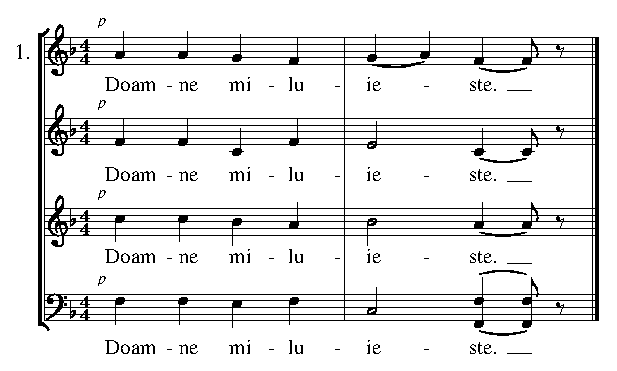
\epsfig{file=dm_1.eps}
    \end{center}
  \end{figure}

  {\bf Preotul:} Pentru bun\u{a} \^{i}ntocmirea aerului, pentru
  \^{i}mbel\c{s}ugarea roadelor p\u{a}m\^{a}ntului \c{s}i pentru
  vremuri pa\c{s}nice, Domnului s\u{a} ne rug\u{a}m.

  {\bf Cantorul:}
  \begin{figure}[h]
    \begin{center}
      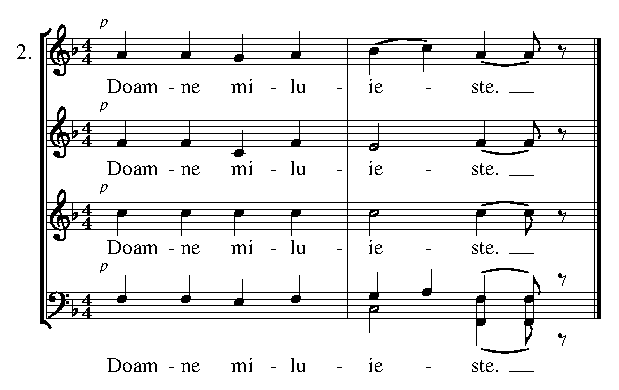
\epsfig{file=dm_2.eps}
    \end{center}
  \end{figure}

  \pagebreak

  {\bf Preotul:} Pentru cei ce c\u{a}l\u{a}toresc pe ape, pe uscat
  \c{s}i prin aer, pentru cei bolnavi, pentru cei robi\c{t}i \c{s}i
  pentru m\^{a}ntuirea lor, Domnului s\u{a} ne rug\u{a}m.

  {\bf Cantorul:}
  \begin{figure}[h]
    \begin{center}
      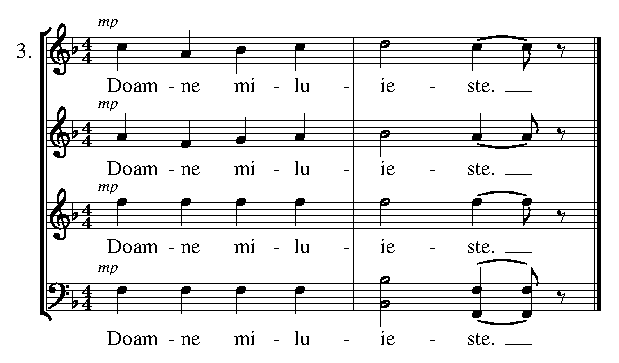
\epsfig{file=dm_3.eps}
    \end{center}
  \end{figure}

  {\bf Preotul:} Pentru ca s\u{a} fim izb\u{a}vi\c{t}i noi de tot
  necazul, m\^{a}nia, primejdia \c{s}i nevoia, Domnului s\u{a} ne
  rug\u{a}m.

  {\bf Cantorul:}
  \begin{figure}[h]
    \begin{center}
      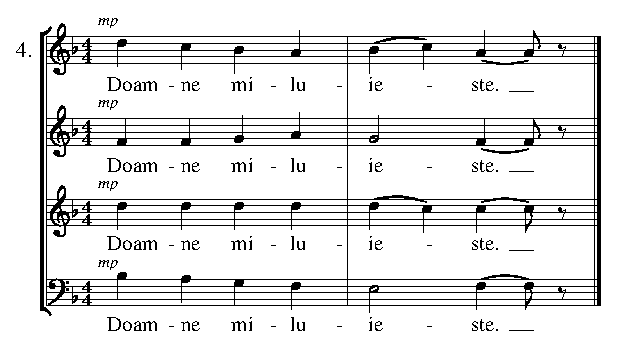
\epsfig{file=dm_4.eps}
    \end{center}
  \end{figure}

  \pagebreak

  {\bf Preotul:} Ap\u{a}r\u{a}, m\^{a}ntuie\c{s}te, miluie\c{s}te
  \c{s}i ne p\u{a}ze\c{s}te pe noi, Dumnezeule, cu harul T\u{a}u.

  {\bf Cantorul:}
  \begin{figure}[h]
    \begin{center}
      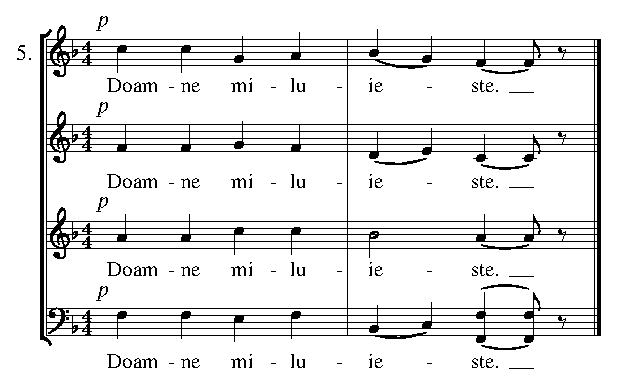
\epsfig{file=dm_5.eps}
    \end{center}
  \end{figure}

  {\bf Preotul:} Pe preasf\^{a}nta, curata, prea binecuv\^{a}ntata,
  m\u{a}rita St\u{a}p\^{a}na noastr\u{a}, de Dumnezeu
  N\u{a}sc\u{a}toarea \c{s}i pururea Fecioara Maria, cu to\c{t}i
  sfin\c{t}ii s\u{a} o pomenim.

  {\bf Cantorul:}
  \begin{figure}[h]
    \begin{center}
      \epsfig{file=prea_sfanta_nascatoare.eps}
    \end{center}
  \end{figure}

  \pagebreak

  {\bf Preotul:} Pe noi \^{i}n\c{s}ine \c{s}i unii pe al\c{t}ii
  \c{s}i toat\u{a} via\c{t}a noastr\u{a} lui Hristos Dumnezeu s\u{a} o
  d\u{a}m.

  {\bf Cantorul:}
  \begin{figure}[h]
    \begin{center}
      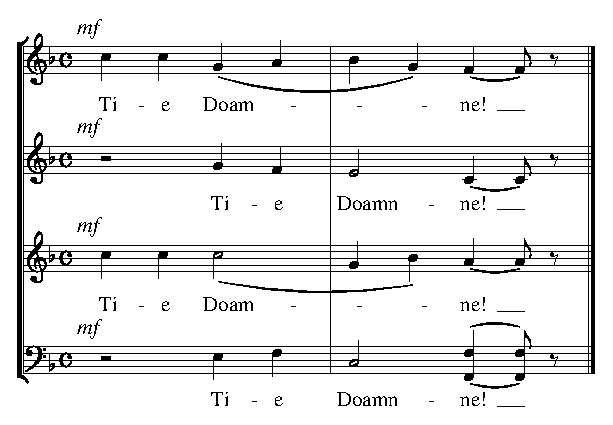
\epsfig{file=tie_doamne.eps}
    \end{center}
  \end{figure}

  {\bf Preotul:} C\u{a} \c{T}ie se cuvinte toat\u{a} m\u{a}rirea,
  cinstea \c{s}i \^{i}nchin\u{a}ciunea, Tat\u{a}lui \c{s}i Fiului
  \c{s}i Sf\^{a}ntului Duh, acum \c{s}i pururea \c{s}i \^{i}n vecii
  vecilor.

  {\bf Cantorul:}
  \begin{figure}[h]
    \begin{center}
      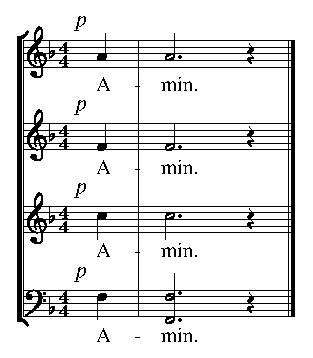
\epsfig{file=amin_2.eps}
    \end{center}
  \end{figure}

  \pagebreak

  \begin{center}
    {\large \bf ANTIFONUL I\\
      Glas 8}
  \end{center}

  \begin{figure}[h]
    \begin{center}
      \epsfig{file=antifonul_1-page1.eps}
    \end{center}
  \end{figure}

  \pagebreak

  \begin{figure}[h]
    \begin{center}
      \epsfig{file=antifonul_1-page2.eps}
    \end{center}
  \end{figure}

  \pagebreak

  \begin{center}
    {\large \bf ECTENIA MIC\u{A}\\
      Glas 8}
  \end{center}

  {\bf Preotul:} Iar\u{a} \c{s}i iar\u{a} cu pace, Domnului s\u{a} ne
  rug\u{a}m.

  {\bf Cantorul:}
  \begin{figure}[h]
    \begin{center}
      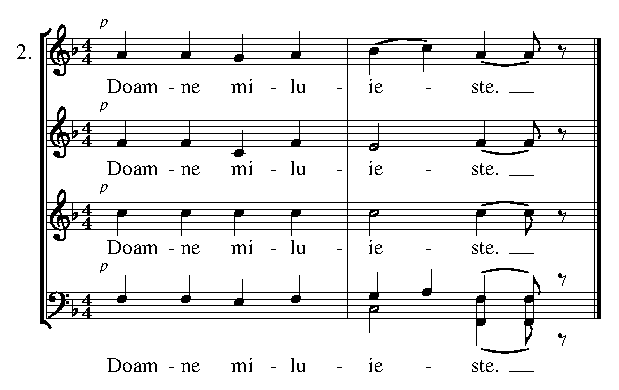
\epsfig{file=dm_2.eps}
    \end{center}
  \end{figure}

  {\bf Preotul:} Ap\u{a}r\u{a}, m\^{a}ntuie\c{s}te, miluie\c{s}te
  \c{s}i ne p\u{a}ze\c{s}te pe noi, Dumnezeule, cu harul T\u{a}u.

  {\bf Cantorul:}
  \begin{figure}[h]
    \begin{center}
      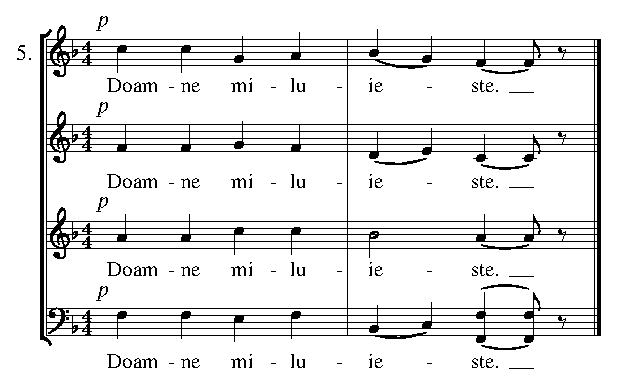
\epsfig{file=dm_5.eps}
    \end{center}
  \end{figure}

  \pagebreak

  {\bf Preotul:} Pe preasf\^{a}nta, curata, prea binecuv\^{a}ntata,
  m\u{a}rita St\u{a}p\^{a}na noastr\u{a}, de Dumnezeu
  N\u{a}sc\u{a}toarea \c{s}i pururea Fecioara Maria, cu to\c{t}i
  sfin\c{t}ii s\u{a} o pomenim.

  {\bf Cantorul:}
  \begin{figure}[h]
    \begin{center}
      \epsfig{file=prea_sfanta_nascatoare.eps}
    \end{center}
  \end{figure}

  {\bf Preotul:} Pe noi \^{i}n\c{s}ine \c{s}i unii pe al\c{t}ii
  \c{s}i toat\u{a} via\c{t}a noastr\u{a} lui Hristos Dumnezeu s\u{a} o
  d\u{a}m.

  {\bf Cantorul:}
  \begin{figure}[h]
    \begin{center}
      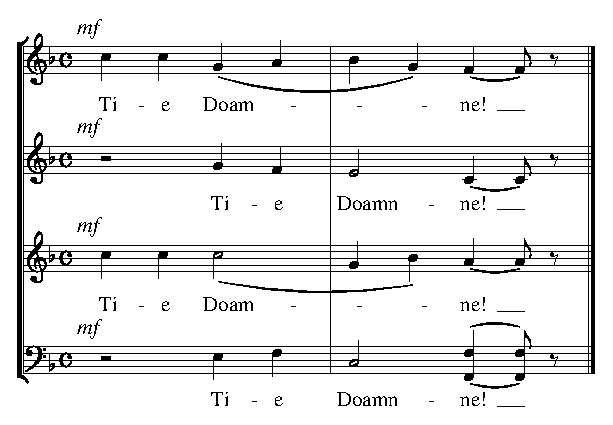
\epsfig{file=tie_doamne.eps}
    \end{center}
  \end{figure}

  \pagebreak

  {\bf Preotul:} C\u{a} a Ta este st\u{a}p\^{a}nirea \c{s}i a Ta este
  \^{i}mp\u{a}r\u{a}\c{t}ia \c{s}i puterea \c{s}i m\u{a}rirea, a
  Tat\u{a}lui \c{s}i a Fiului \c{s}i a Sf\^{a}ntului Duh, acum \c{s}i
  pururea \c{s}i \^{i}n vecii vecilor.

  {\bf Cantorul:}
  \begin{figure}[ht]
    \begin{center}
      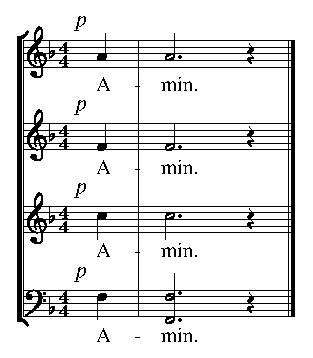
\epsfig{file=amin_2.eps}
    \end{center}
  \end{figure}

  \begin{center}
    {\large \bf ANTIFONUL AL II-lea\\
      Glas 8}
  \end{center}

  \begin{figure}[h]
    \begin{center}
      \epsfig{file=antifonul_2-page1.eps}
    \end{center}
  \end{figure}

  \pagebreak

  \begin{figure}[h]
    \begin{center}
      \epsfig{file=antifonul_2-page2.eps}
    \end{center}
  \end{figure}

  \pagebreak

\end{document}
